\begin{usecase}{View Integrated Calendar}
  \ucbasicinfo{High}{Regular}
  \ucshortdescription{Allows users to view their integrated calendar}
  \uctrigger{User selects the option to view the integrated calendar.}
  \ucactors{User}{None}
  \ucpreconditions{User must be logged into the system.}
  \ucrelationships{N/A}{N/A}{N/A}
  \ucinputsoutputs{
    \begin{itemize}
      \item \textbf{Integrated calendar} (Source: System)
    \end{itemize}
  }{
    \begin{itemize}
      \item \textbf{Integrated calendar} (Destination: App)
    \end{itemize}
  }
  \ucmainflow{
    \begin{enumerate}
      \item The user clicks on the integrated calendar.
            \ucinfo{The system displays the all integrated calendars and it's events}
    \end{enumerate}
  }
  \ucconclusion{User successfully views their integrated calendar with all the events.}
  \ucpostconditions{The integrated calendar is displayed}
  \ucspecialrequirements{N/A}
  \ucbusinessrules{
    \begin{itemize}
      \item \textbf{Events must be displayed according to user preferences .}
    \end{itemize}
  }
\end{usecase}

\begin{figure}[!h]
  \centering
  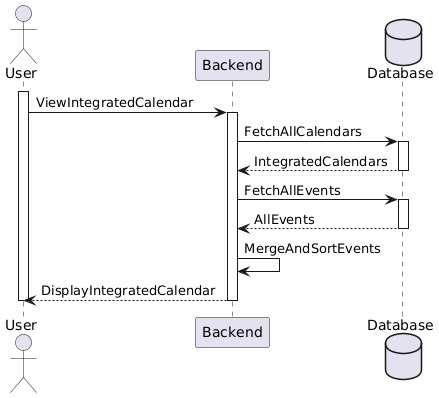
\includegraphics[width=\textwidth]{images/docs/diagrams/sequence-diagrams/all-sequence-diagrams/View Integrated Calendar.png}
  \caption{View Integrated Calendar Sequence Diagram}
  \label{fig:seq/view-integrated-calendar}
\end{figure}

The "View Integrated Calendar Sequence Diagram", shown in \textbf{Figure~\ref{fig:seq/view-integrated-calendar}}, demonstrates the process of presenting a unified view of all connected calendars to the user. The sequence begins when the user initiates a ViewIntegratedCalendar gRPC call to access their comprehensive calendar view.

The Backend executes a two-phase data retrieval process:
\begin{enumerate}
  \item First queries the Database via FetchAllCalendars to retrieve all calendar sources connected to the user's account
  \item Then executes FetchAllEvents to gather events from all calendars
\end{enumerate}

After data retrieval, the Backend performs critical processing:
\begin{itemize}
  \item Merges events from different calendar sources
  \item Sorts events chronologically
  \item Applies user preferences for event display
\end{itemize}

Finally, the Backend returns the processed calendar data through the gRPC channel as DisplayIntegratedCalendar response. This unified view ensures users can efficiently manage their schedule across all connected calendars, maintaining consistency with user preferences while providing a comprehensive overview of all commitments.